% ==========================================
% فایل: steps/step03.tex
% گام ۳: یافتن تمامی تناظرها بین نقاط
% ==========================================

\section{گام (۳): استخراج تناظرها و تحلیل داده‌های پرت}

\begin{stepbox}
\field{روند کار و اعمال فیلترهای تطابق}{
برای پیدا کردن جفت‌نقاط متناظر بین دو تصویر، از تطبیق‌دهنده‌ی \lr{Brute-Force} استفاده کردیم. از آنجایی که الگوریتم به صورت پیش‌فرض ممکن است یک نقطه از تصویر اول را به چندین نقطه شبیه به هم در تصویر دوم متصل کند، دو فیلتر مهم را برای افزایش دقت پیاده‌سازی کردیم:
\begin{itemize}
    \item \textbf{فیلتر اول (\lr{Cross-Check}):} این فیلتر تضمین می‌کند که نقطه‌ی $A$ در تصویر اول تنها در صورتی با نقطه‌ی $B$ در تصویر دوم جفت می‌شود که این رابطه دوطرفه باشد (یعنی $A$ نزدیک‌ترین همسایه برای $B$ و بالعکس باشد).
    \item \textbf{فیلتر دوم (\lr{Distance Threshold}):} با اعمال یک حد آستانه برای فاصله‌ی اقلیدسی بین بردارها، تناظرهایی که شباهت کمی دارند (فاصله‌شان زیاد است) حذف می‌شوند.
\end{itemize}
}

\begin{codebox}[یافتن تناظرها با الگوریتم Brute-Force]
\begin{lstlisting}[language=Python]
# 1. Initialize BFMatcher with L2 norm and cross-check enabled
bf = cv2.BFMatcher(cv2.NORM_L2, crossCheck=True)

# 2. Match descriptors between image 1 and image 2
matches = bf.match(des1, des2)

# 3. Sort matches based on distance (lower distance = higher similarity)
matches = sorted(matches, key=lambda x: x.distance)

# 4. Keep only good matches by applying a distance threshold
distance_threshold = 150
good_matches = [m for m in matches if m.distance < distance_threshold]
\end{lstlisting}
\end{codebox}

\field{تحلیل بصری نتایج و شناسایی \lr{Outliers}}{
با رسم خطوطِ متصل‌کننده بین نقاطِ فیلتر شده، متوجه یک چالش اساسی در پردازش تصویر می‌شویم. در حالت ایده‌آل (چون دوربین صرفاً در یک صفحه جابه‌جا شده است)، تمامی خطوط باید موازی باشند. اما در خروجی‌های به دست آمده:
\begin{itemize}
    \item \textbf{مجموعه اول:} خطوط متقاطع زیادی دیده می‌شود که به دلیل تشابه کاراکترهای متنی روی وایت‌برد و لبه‌های کتاب‌ها به وجود آمده است.
    \item \textbf{مجموعه دوم:} شاخ و برگ متراکم درختان باعث فریب خوردن الگوریتم و ایجاد خطوط مورب (\lr{Outliers}) شده است.
    \item \textbf{مجموعه سوم:} بافتِ به شدت تکرارشونده‌ی موکتِ کف اتاق، باعث شده تا برخی نقاط به اشتباه با نقطه‌ای دیگر در چند سانتی‌متری خود مچ شوند.
\end{itemize}
وجود این خطاهای تطبیق (که حدود ۲۰ الی ۳۰ درصد از کل تناظرها را شامل می‌شوند) کاملاً طبیعی است و ضرورت استفاده از یک مدل هندسیِ مقاوم به داده‌های پرت (مانند \lr{RANSAC}) در گام بعدی را توجیه می‌کند.
}
\end{stepbox}

\begin{figure}[h!]
    \centering
    \begin{subfigure}{0.48\textwidth}
        \centering
        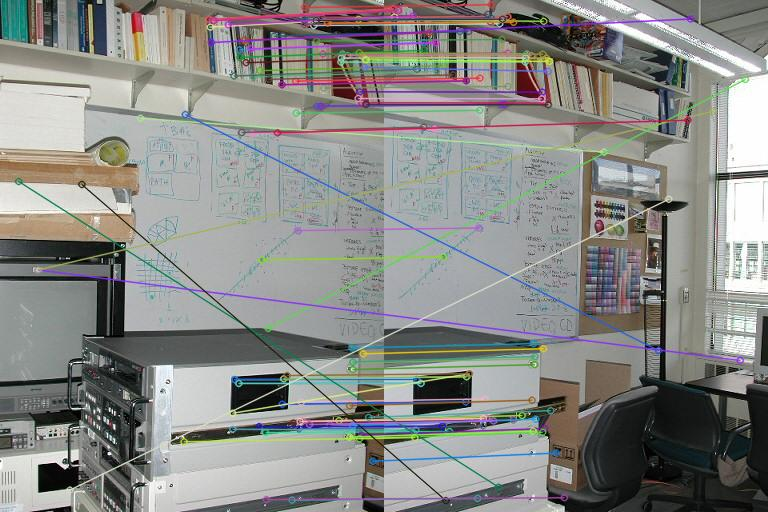
\includegraphics[width=\textwidth]{images/Part_3/Matches_1.jpg}
        \caption{مجموعه اول: خطای تطبیق ناشی از متون و کتاب‌ها}
    \end{subfigure}
    \hfill
    \begin{subfigure}{0.48\textwidth}
        \centering
        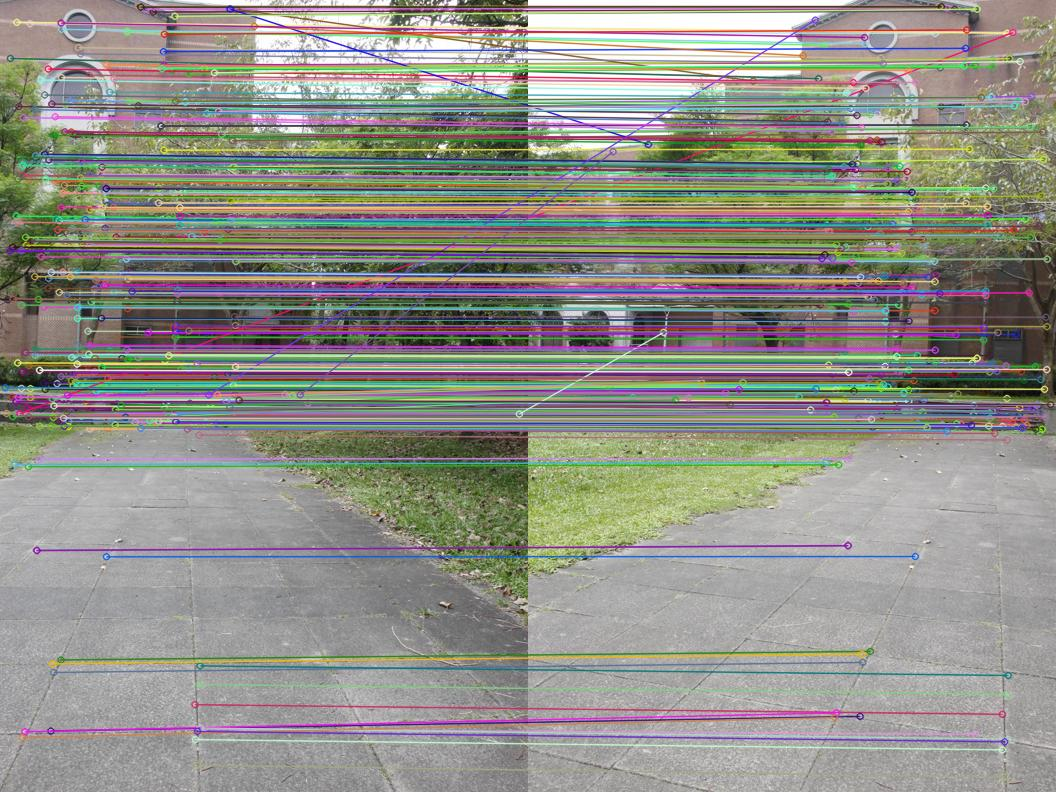
\includegraphics[width=\textwidth]{images/Part_3/Matches_2.jpg}
        \caption{مجموعه دوم: خطاهای مورب ناشی از شاخ و برگ درختان}
    \end{subfigure}
    
    \vspace{0.4cm}
    \begin{subfigure}{0.6\textwidth}
        \centering
        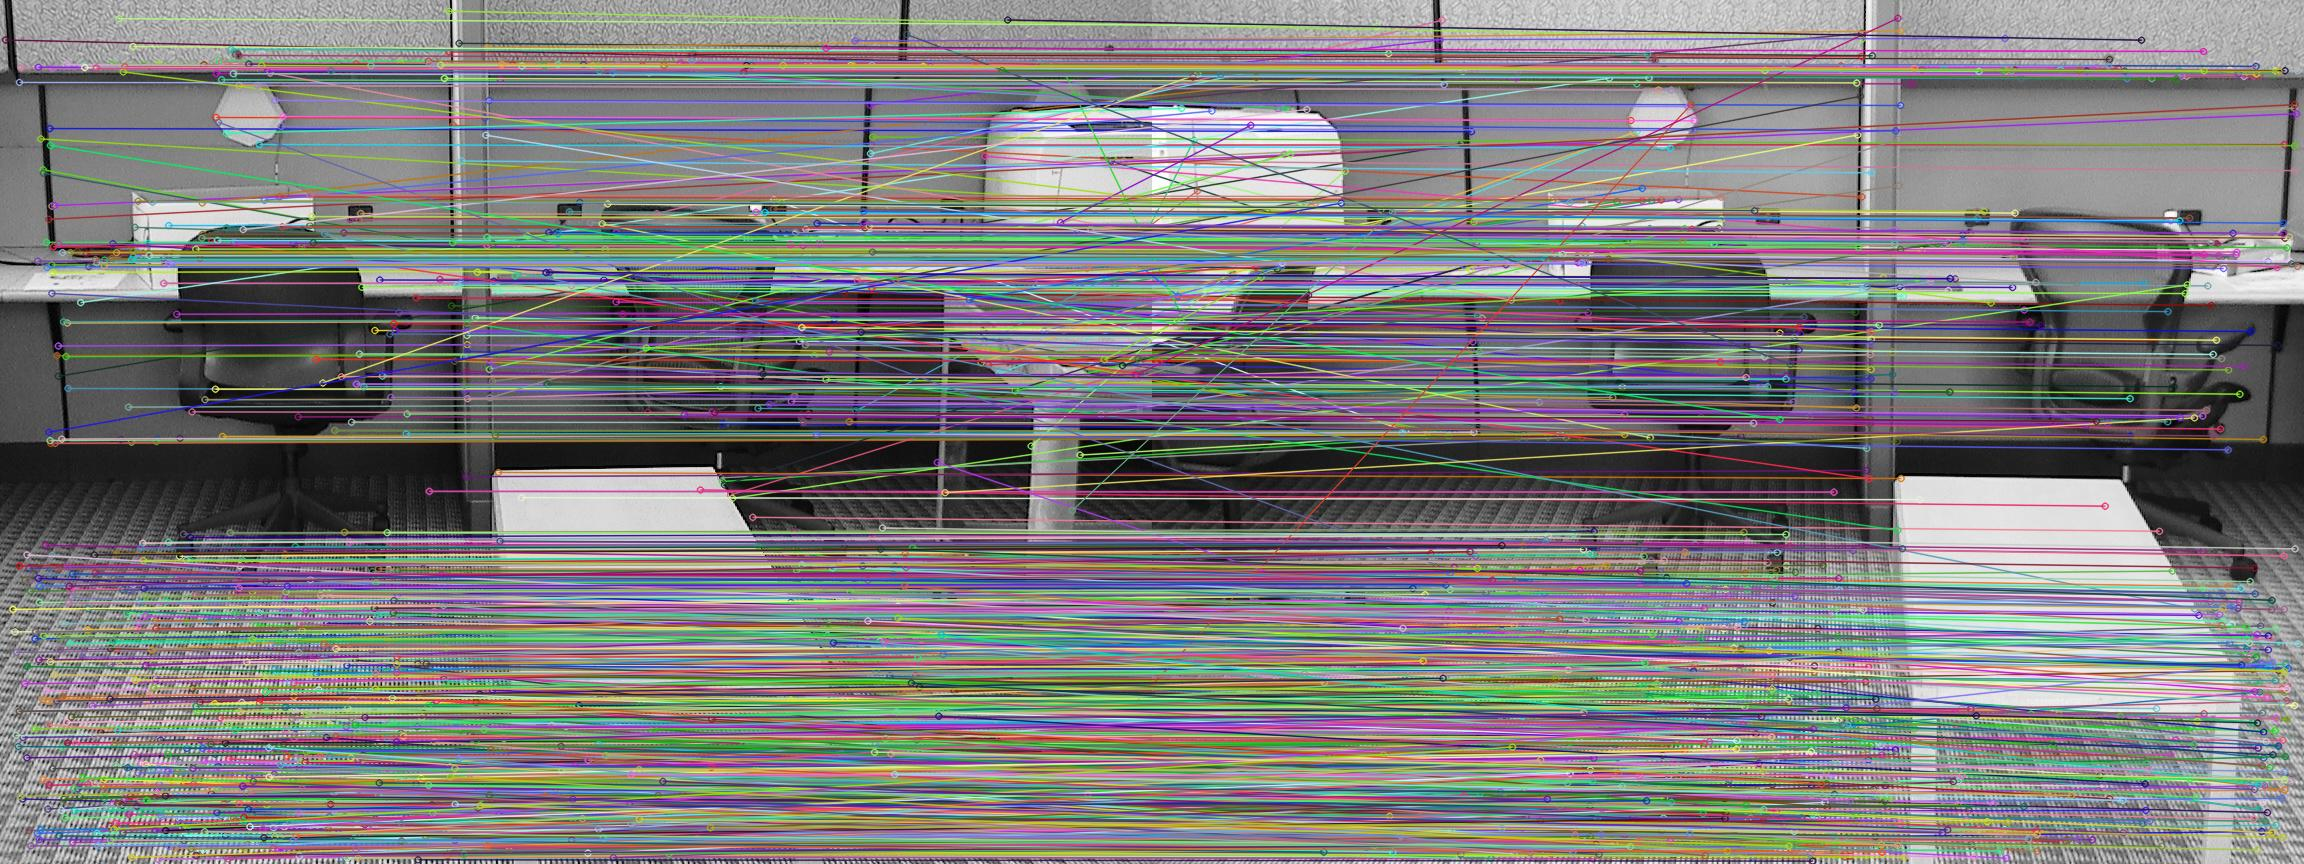
\includegraphics[width=\textwidth]{images/Part_3/Matches_3.jpg}
        \caption{مجموعه سوم: تراکم بالا و خطاهای ناشی از بافت تکراری موکت}
    \end{subfigure}
    \caption{بررسی چالش‌های تطبیق ویژگی‌ها؛ خطوط غیرموازی نمایانگر داده‌های پرت (\lr{Outliers}) هستند.}
\end{figure}